%%%%%%%%%%%%%%%%%%%%%%%%%%%%%%%%%%%%%%%%%%%%%%%%%%%%%%%%%%%%%%%%%%%%%%
% How to use writeLaTeX: 
%
% You edit the source code here on the left, and the preview on the
% right shows you the result within a few seconds.
%
% Bookmark this page and share the URL with your co-authors. They can
% edit at the same time!
%
% You can upload figures, bibliographies, custom classes and
% styles using the files menu.
%
%%%%%%%%%%%%%%%%%%%%%%%%%%%%%%%%%%%%%%%%%%%%%%%%%%%%%%%%%%%%%%%%%%%%%%

% chktex-file 44

\documentclass[12pt]{article}

\usepackage{sbc-template}

\usepackage{graphicx,url}

\usepackage[brazil]{babel}
\usepackage[utf8]{inputenc}

\usepackage{listings}
\usepackage{xcolor}
\usepackage{float}
\usepackage{amsmath} 
\usepackage{tikz}
\usepackage{subfigure}
\usepackage{float}

% Definição de cores personalizadas
\definecolor{mygreen}{rgb}{0,0.6,0}        % Para comentários
\definecolor{mygray}{rgb}{0.5,0.5,0.5}       % Para números de linha
\definecolor{mymauve}{rgb}{0.58,0,0.82}       % Para strings
\definecolor{myblue}{rgb}{0,0,0.8}            % Para palavras-chave
\definecolor{lightgray}{rgb}{0.95,0.95,0.95}  % Fundo dos códigos

% Configuração padrão para todos os códigos
\lstset{
  backgroundcolor=\color{lightgray},
  basicstyle=\ttfamily\footnotesize,
  breaklines=true,
  captionpos=b,
  numbers=left,
  numberstyle=\tiny\color{mygray},
  frame=single,
  keywordstyle=\color{myblue}\bfseries,
  commentstyle=\color{mygreen}\itshape,
  stringstyle=\color{mymauve},
  tabsize=4,
  showstringspaces=false,
  aboveskip=10pt,
  belowskip=5pt
}
% Estilo para código em C
\lstdefinestyle{CStyle}{
  language=C,
  % Outras opções específicas para C podem ser adicionadas aqui
}

% Definindo uma linguagem para CUDA baseada em C++
\lstdefinelanguage{CUDA}[]{C++}{
  morekeywords={__global__, __device__, __shared__, __host__},
  % Caso necessário, adicione mais palavras-chave ou opções específicas
}

% Estilo para código em Python
\lstdefinestyle{PythonStyle}{
  language=Python,
  morekeywords=[2]{SequentialDiffusionEquation,with,OMPdiffusionEquation,CUDADiffusionEquation},
  % Outras opções específicas para Python podem ser adicionadas aqui
}

\renewcommand{\lstlistingname}{Código}

\sloppy

\title{Engane a IA: Desenvolvendo Perturbações Adversariais Contra Classificadores de DeepFake}

\author{Eduardo Verissimo Faccio, Guilherme Ferreira Lourenço}

\address{Instituto de Ciência e Tecnologia -- Universidade Federal de São Paulo
  (UNIFESP)\\
  São José dos Campos -- SP -- Brasil
  \email{\{verissimo.eduardo,gflourenco\}@unifesp.br}
}

\begin{document}

\maketitle

\begin{resumo}
    Este trabalho explora a vulnerabilidade e a robustez de redes neurais diante de ataques adversariais
    imperceptíveis aos humanos. Utilizando a base de dados “140k Real and Fake Faces”, treinou-se uma rede
    neural convolucional, uma mini UNET e um XGBoost para a classificação de imagens faciais, atingindo alta
    acurácia em condições normais. Em seguida, desenvolveu-se um ataque adversarial baseado em uma arquitetura
    UNET, capaz de gerar perturbações sutis que comprometem significativamente o desempenho do classificador.
    Os resultados demonstram que, mesmo com perturbações invisíveis a olho nu, a confiabilidade dos sistemas de reconhecimento
    facial pode ser severamente comprometida, ressaltando a importância de desenvolver estratégias para aumentar
    a resiliência dos classificadores.

    \textbf{Palavras-chave}: Ataques adversariais, robustez, redes neurais convolucionais, perturbações imperceptíveis, reconhecimento facial, XGBoost.
\end{resumo}

\section{Introdução}

O avanço das técnicas de aprendizado profundo tem permitido que sistemas de
reconhecimento facial alcancem níveis de acurácia sem precedentes, contribuindo
para uma ampla gama de aplicações, desde segurança pública até interfaces de
usuário baseadas em biometria~\cite{parkhi2015deep}. Entretanto, apesar do
desempenho elevado, diversos estudos demonstraram que redes neurais são
inerentemente vulneráveis a perturbações adversariais - pequenas modificações
imperceptíveis a olho nu que podem levar a classificações
equivocadas~\cite{szegedy2014intriguingpropertiesneuralnetworks,goodfellow2015explainingharnessingadversarialexamples}.

Neste contexto, o presente trabalho investiga a robustez de modelos de
classificação de imagens faciais quando expostos a ataques adversariais sutis.
Utilizando a base de dados ``140k Real and Fake Faces'', foram treinados três
classificadores distintos - uma rede neural convolucional (CNN), uma versão
reduzida de UNET \cite{ronneberger2015u} e um classificador baseado em
XGBoost~\cite{Chen_2016} a - que, sob condições normais, alcançaram alto
desempenho. Em seguida, propõe-se um ataque adversarial que se baseia em uma
arquitetura UNET parecida com o classificador criado, cujo objetivo é gerar
perturbações imperceptíveis que comprometam a confiabilidade dos
classificadores.

Ao integrar modelos de naturezas distintas na análise, este estudo busca
identificar possíveis diferenças na robustez dos sistemas frente a ataques
adversariais, evidenciando as limitações dos métodos de classificação atuais e
a necessidade de desenvolver estratégias defensivas que aumentem a resiliência
dos sistemas de reconhecimento facial. A abordagem proposta não só contribui
para uma compreensão mais aprofundada das vulnerabilidades dos modelos de
aprendizado profundo, mas também sugere caminhos para a implementação de
mecanismos de defesa que possam mitigar os impactos desses ataques em
aplicações críticas.

\section{Referencial Teórico}
\subsection{Redes Neurais Convolucionais e Reconhecimento Facial}
Redes neurais convolucionais (CNNs) têm se destacado no processamento de
imagens devido à sua capacidade de extrair automaticamente características
hierárquicas, desde padrões simples, como bordas e texturas, até estruturas
complexas, essenciais para o reconhecimento facial. Estudos como o de Parkhi et
al. (2015) demonstram que a utilização de arquiteturas profundas permite
alcançar altos índices de acurácia, tornando as CNNs a escolha preferencial
para aplicações em biometria.

\subsection{Ataques Adversariais}
Apesar do elevado desempenho, as CNNs são vulneráveis a perturbações
adversariais - pequenas modificações intencionais e imperceptíveis na entrada
que podem levar a classificações errôneas. Szegedy et al. (2013) foram
pioneiros ao evidenciar essa fragilidade, enquanto Goodfellow et al. (2014)
apresentaram o Fast Gradient Sign Method (FGSM) para gerar tais perturbações.
Esses ataques exploram a alta dimensionalidade dos dados e a complexidade dos
espaços de decisão dos modelos, comprometendo a confiabilidade dos sistemas de
reconhecimento facial.

\subsection{Estratégias de Geração de Perturbações}
Diversas técnicas de ataque adversarial têm sido propostas, baseadas na
otimização da função de perda do modelo. Entre elas, o FGSM e suas variações
mostram alta eficácia na geração de exemplos adversariais. Neste trabalho,
adota-se uma abordagem que utiliza uma arquitetura UNET para criar perturbações
sutis. A escolha da UNET como base se justifica por sua capacidade comprovada
de capturar detalhes contextuais e preservar informações espaciais,
características que foram originalmente exploradas por Ronneberger et al.
(2015) em seu trabalho. Adaptamos essa estrutura para garantir que as
modificações permaneçam num intervalo pré-definido (por exemplo,
[$-\epsilon$,$\epsilon$]), assegurando que as perturbações sejam imperceptíveis
ao olho humano, mas capazes de degradar significativamente o desempenho dos
classificadores.

\subsection{Outros Classificadores e Robustez dos Modelos}
Além das CNNs, outros classificadores, como UNET e o XGBoost, têm sido
empregados em problemas de classificação de imagens.

A versão reduzida da UNET utilizada neste trabalho deriva do modelo
originalmente proposto por Ronneberger para segmentação de imagens biomédicas,
demonstrando alta eficiência na extração de características relevantes
\cite{ronneberger2015u}. Esse modelo revolucionou o campo da segmentação de
imagens ao demonstrar que uma rede com caminhos de contração e expansão, aliada
a conexões de \textit{skip}, pode extrair e preservar informações espaciais
cruciais.

O XGBoost, conforme descrito por Chen Guestrin (2016), utiliza técnicas de
boosting que o tornam robusto e eficiente, especialmente em cenários com dados
de alta dimensionalidade.

A comparação entre esses modelos permite avaliar a variabilidade na robustez
frente a ataques adversariais, demonstrando que, mesmo que a mesma perturbação
seja aplicada, a sensibilidade de cada modelo pode variar, evidenciando a
necessidade de estratégias defensivas que aumentem a resiliência global dos
sistemas de reconhecimento facial.

\subsection{Transferibilidade dos Ataques e Estratégias defensivas}
Um aspecto crítico dos ataques adversariais é a sua capacidade de
transferência, isto é, a perturbação gerada para um modelo pode afetar outros
modelos, mesmo que estes tenham arquiteturas distintas. Essa propriedade
aumenta a ameaça dos ataques em cenários do mundo real, onde o atacante pode
não ter acesso direto ao modelo alvo \cite{tramer2021}. Compreender e mitigar
essa transferência é fundamental para o desenvolvimento de mecanismos de defesa
robustos que assegurem a integridade dos sistemas de reconhecimento facial em
ambientes críticos.

\section{Metodologia}

A abordagem adotada neste trabalho visa investigar a robustez de
classificadores de imagens faciais frente a ataques adversariais
imperceptíveis. Para isso, a metodologia foi dividida em três etapas
principais: (i) preparação e treinamento dos modelos, (ii) desenvolvimento do
ataque adversarial e (iii) avaliação dos resultados.

\subsection{Preparação dos Dados e Treinamento dos Modelos}

A base de dados utilizada foi a \textit{``140k Real and Fake Faces''}, composta
por imagens reais e geradas, que foram previamente divididas em conjuntos de
treinamento, validação e teste. A seguir, três modelos foram treinados para a
classificação de imagens faciais:

\begin{itemize}
    \item \textbf{Rede Neural Convolucional (CNN):} Implementada em PyTorch, esta arquitetura
          é composta por camadas convolucionais, seguidas por camadas de pooling, normalização e
          camadas totalmente conectadas.

          \begin{figure}[htbp]
              \centering

              \begin{tikzpicture}[scale=0.5, transform shape, node distance=1.5cm, auto]
                  % Nodes for CNN
                  \node [draw, rectangle, align=center] (inputcnn) {Input\\(128x128x3)};
                  \node [draw, rectangle, align=center, below of=inputcnn] (conv1) {Conv 1\\(3$\to$32)};
                  \node [draw, rectangle, align=center, below of=conv1] (pool1) {Max Pool};
                  \node [draw, rectangle, align=center, below of=pool1] (conv2) {Conv 2\\(32$\to$64)};
                  \node [draw, rectangle, align=center, below of=conv2] (pool2) {Max Pool};
                  \node [draw, rectangle, align=center, below of=pool2] (conv3) {Conv 3\\(64$\to$128)};
                  \node [draw, rectangle, align=center, below of=conv3] (pool3) {Max Pool};
                  \node [draw, rectangle, align=center, below of=pool3] (conv4) {Conv 4\\(128$\to$256)};
                  \node [draw, rectangle, align=center, below of=conv4] (pool4) {Max Pool};
                  \node [draw, rectangle, align=center, below of=pool4] (global) {Global Avg Pool};
                  \node [draw, rectangle, align=center, below of=global] (fc1) {FC 1};
                  \node [draw, rectangle, align=center, below of=fc1] (fc2) {FC 2};
                  \node [draw, rectangle, align=center, below of=fc2] (fc3) {FC 3\\(2 classes)};

                  % Arrows for CNN
                  \draw [->] (inputcnn) -- (conv1);
                  \draw [->] (conv1) -- (pool1);
                  \draw [->] (pool1) -- (conv2);
                  \draw [->] (conv2) -- (pool2);
                  \draw [->] (pool2) -- (conv3);
                  \draw [->] (conv3) -- (pool3);
                  \draw [->] (pool3) -- (conv4);
                  \draw [->] (conv4) -- (pool4);
                  \draw [->] (pool4) -- (global);
                  \draw [->] (global) -- (fc1);
                  \draw [->] (fc1) -- (fc2);
                  \draw [->] (fc2) -- (fc3);
              \end{tikzpicture}
              \caption{Diagrama da arquitetura da CNN.}
          \end{figure}

    \item \textbf{Mini UNET:} Uma versão reduzida da tradicional arquitetura UNET foi
          desenvolvida para explorar sua capacidade em extrair características e classificar as
          imagens, mantendo uma complexidade computacional inferior.

          \begin{figure}[htbp]
              \centering
              \begin{tikzpicture}[scale=0.5, transform shape, node distance=1.5cm, auto]
                  % Encoder Path
                  \node [draw, rectangle, align=center] (input) {Input\\(128x128x3)};
                  \node [draw, rectangle, align=center, below of=input] (enc1) {Enc1: Conv Block\\(32, 128x128)};
                  \node [draw, rectangle, align=center, below of=enc1] (pool1) {Max Pool\\(32, 64x64)};
                  \node [draw, rectangle, align=center, below of=pool1] (enc2) {Enc2: Conv Block\\(64, 64x64)};
                  \node [draw, rectangle, align=center, below of=enc2] (pool2) {Max Pool\\(64, 32x32)};
                  \node [draw, rectangle, align=center, below of=pool2] (bottleneck) {Bottleneck: Conv Block\\(128, 32x32)};

                  % Decoder Path (posicionado à direita)
                  \node [draw, rectangle, align=center, right of=bottleneck, right=1.5cm] (up1) {UpConv1\\(64, 64x64)};
                  \node [draw, rectangle, align=center, above of=up1, above=0.9cm] (dec1) {Dec1: Conv Block\\(64, 64x64)};
                  \node [draw, rectangle, align=center, right of=dec1, right=1cm] (up2) {UpConv2\\(32, 128x128)};
                  \node [draw, rectangle, align=center, above of=up2, above=0.9cm] (dec2) {Dec2: Conv Block\\(32, 128x128)};

                  % Classification Head
                  \node [draw, rectangle, align=center, right of=dec2, right=1cm] (global) {Global Avg Pool\\(32, 1x1)};
                  \node [draw, rectangle, align=center, below of=global, below=1cm] (fc) {FC\\(2 classes)};

                  % Arrows for Encoder
                  \draw [->] (input) -- (enc1);
                  \draw [->] (enc1) -- (pool1);
                  \draw [->] (pool1) -- (enc2);
                  \draw [->] (enc2) -- (pool2);
                  \draw [->] (pool2) -- (bottleneck);

                  % Arrows for Decoder
                  \draw [->] (bottleneck) -- (up1);
                  \draw [->] (up1) -- (dec1);
                  \draw [->] (dec1) -- (up2);
                  \draw [->] (up2) -- (dec2);
                  \draw [->] (dec2) -- (global);
                  \draw [->] (global) -- (fc);

                  % Skip connections
                  \draw [->, dashed] (enc2.east) -- ++(1,0) |- (dec1.west);
                  \draw [->, dashed] (enc1.east) -- ++(1,0) |- (dec2.west);
              \end{tikzpicture}
              \caption{Diagrama da arquitetura da Mini UNET.}
              \label{fig:mini_unet}
          \end{figure}

    \item \textbf{XGBoost:} Utilizando o framework XGBoost~\cite{Chen_2016}, foi treinado
          um classificador baseado em boosting, que se mostrou eficiente para problemas de alta
          dimensionalidade.
\end{itemize}

Todos os modelos foram treinados sob condições normais, atingindo altos índices
de acurácia no conjunto de teste.

\subsection{Desenvolvimento do Ataque Adversarial}

Após o treinamento dos classificadores, desenvolveu-se um ataque adversarial
visando gerar perturbações sutis e imperceptíveis que comprometem a
confiabilidade dos modelos. Para isso, foi utilizada uma arquitetura UNET,
denominada rede adversarial, que recebe como entrada uma imagem normalizada (em
escala \([-1, 1]\)) e gera uma perturbação. Essa perturbação é então limitada
por um mecanismo de \textit{clamp}, para garantir que as alterações não excedam
um intervalo pré-definido \([-\epsilon, \epsilon]\). Formalmente, a imagem
adversarial \( \text{adv\_x} \) é obtida através da equação:

\[
    \text{adv\_x} = \text{clamp}\Bigl(x + \text{clamp}\bigl(\text{Perturbação}(x), -[\epsilon], [\epsilon]\bigr), -1, 1\Bigr)
\]

onde \( x \) representa a imagem original. Essa abordagem assegura que as
modificações sejam imperceptíveis ao olho humano, mas capazes de induzir erros
nos classificadores.
\begin{figure}[htbp]
    \centering
    \begin{tikzpicture}[scale=0.5, transform shape, node distance=1.5cm, auto]
        % Nodes for adversarial network
        \node [draw, rectangle, align=center] (input) {Input\\(128x128x3)};
        \node [draw, rectangle, align=center, below of=input] (down1) {DownBlock 1\\(128$\to$64)};
        \node [draw, rectangle, align=center, below of=down1] (down2) {DownBlock 2\\(64$\to$32)};
        \node [draw, rectangle, align=center, below of=down2] (bottleneck) {Residual Block};
        \node [draw, rectangle, align=center, below of=bottleneck] (up1) {UpBlock 1\\(32$\to$64)};
        \node [draw, rectangle, align=center, below of=up1] (up2) {UpBlock 2\\(64$\to$128)};
        \node [draw, rectangle, align=center, below of=up2] (final) {Final Conv\\(128x128x3)};

        % Arrows for adversarial network
        \draw [->] (input) -- (down1);
        \draw [->] (down1) -- (down2);
        \draw [->] (down2) -- (bottleneck);
        \draw [->] (bottleneck) -- (up1);
        \draw [->] (up1) -- (up2);
        \draw [->] (up2) -- (final);

        % Perturbação: using a tabular to force safe line breaks
        \node [right of=final, xshift=2.5cm, align=center] (clamp) {%
            \begin{tabular}{c}
                Clamp                  \\[2pt]
                $[-\epsilon,\epsilon]$ \\[2pt]
                Perturbação
            \end{tabular}
        };
        \draw [->] (final) -- (clamp);
    \end{tikzpicture}
    \caption{Diagrama da rede adversarial.}
\end{figure}

\subsection{Avaliação Cruzada do Ataque Adversarial}
Além da avaliação convencional dos ataques adversariais, foi realizado um
estudo adicional para investigar a generalização das perturbações geradas pelo
ataque e a eficácia dos ataques adversariais em diferentes contextos. Esse
estudo consiste em treinar a rede adversarial contra um modelo específico e,
posteriormente, testá-la contra outro classificador não visto durante o
treinamento do ataque.

O objetivo dessa abordagem é determinar se as perturbações adversariais são
específicas ao modelo para o qual foram treinadas ou se possuem propriedades
transferíveis, capazes de enganar diferentes arquiteturas de classificação.
Para isso, foi realizado o seguinte procedimento experimental:

Treinamento da rede adversarial para enganar um classificador específico,
escolhendo entre CNN ou UNET. Geração das imagens adversariais utilizando a
rede treinada. Aplicação dessas imagens adversariais no outro classificador
para avaliar o impacto e o desempenho na detecção das imagens modificadas.
Medição da eficácia do ataque por meio de métricas como acurácia, precisão,
recall e F1-score, comparando os resultados pré e pós-ataque em cada cenário.

Com essa avaliação, é possível responder a duas questões fundamentais:

As perturbações adversariais são específicas ao modelo utilizado no
treinamento? As perturbações podem ser generalizadas para outros
classificadores, sugerindo uma vulnerabilidade compartilhada entre diferentes
arquiteturas? Se um ataque treinado contra um modelo não afeta
significativamente outro classificador, isso indica que a adversarial possui um
comportamento fortemente dependente da arquitetura alvo. No entanto, se a
adversarial treinada em um modelo reduz drasticamente a acurácia do outro, isso
sugere a existência de padrões estruturais comuns entre os modelos, tornando-os
vulneráveis a ataques transferíveis.

\subsection{Avaliação dos Resultados}

A robustez dos modelos foi avaliada comparando a acurácia obtida sob condições
normais com a acurácia após a aplicação dos ataques adversariais.
Adicionalmente, a técnica GradCAM foi utilizada para visualizar as regiões de
maior atenção dos modelos, permitindo identificar quais áreas (por exemplo,
olhos e lábios) são mais suscetíveis às
perturbações~\cite{selvaraju2017gradcam}.

A avaliação abrangeu os três classificadores de forma integrada, possibilitando
comparar a sensibilidade de cada modelo frente às perturbações geradas pela
rede adversarial. Os resultados quantitativos (como a redução percentual da
acurácia) e as análises qualitativas (obtidas via GradCAM) forneceram uma visão
abrangente sobre as vulnerabilidades dos sistemas de reconhecimento facial.

\section{Experimentos e Resultados}

\subsection{Configuração Experimental}
Foram realizados experimentos para avaliar a robustez dos três classificadores
(CNN, Mini UNET e XGBoost) sob três condições distintas:

\begin{itemize} \item \textbf{Condições Normais:} Treinamento e avaliação dos modelos sem a aplicação de ataques adversariais.
    \item \textbf{Condições Adversariais:} Avaliação dos modelos após a aplicação do ataque adversarial, que utiliza uma arquitetura UNET modificada para gerar perturbações sutis e imperceptíveis.
    \item \textbf{Condições Cruzadas do Ataque Adversarial:} Treino do ataque adversarial contra um modelo específico e depois aplicado a outro classificador não visto durante seu treinamento. Aplicado aos modelos CNN e Mini UNET.
\end{itemize}

Todos os modelos foram treinados utilizando a base de dados "140k Real and Fake
Faces", que possui 100 mil dados para treino, 20 mil para validação e 20 mil
para teste. Todos os resultados apresentados nas próximas seções foram
calculados utilizando os dados do teste.

Para avaliação do desempenho dos modelos, foram consideradas métricas como
acurácia, precisão, recall e F1-Score. Além disso, técnicas de visualização
(GradCAM) foram empregadas para analisar qualitativamente as regiões de maior
atenção dos modelos.

\subsection{Resultados Quantitativos}
A Tabela~\ref{tab:resultados_quantitativos} apresenta o desempenho dos três
modelos avaliados – CNN, Mini UNET e XGBoost – comparando as acurácias obtidas
em condições normais e após a aplicação dos ataques adversariais. Observa-se
que tanto a CNN quanto a Mini UNET alcançaram acurácias muito elevadas (99.0\%
e 97.56\%, respectivamente) em condições normais, enquanto o XGBoost obteve
desempenho consideravelmente inferior (56.20\%). Entretanto, sob ataque
adversarial, os modelos baseados em redes neurais (CNN e Mini UNET) sofreram
reduções expressivas na acurácia, atingindo 62.78\% e 58.48\%, correspondendo a
reduções de 36.22\% e 39.08\%, respectivamente. Por outro lado, o XGBoost
apresentou uma diminuição mais modesta (redução de 8.20\%), considerando que
sua acurácia base já estava inferior à dos demais.

\begin{table}[htbp]
    \centering
    \caption{Desempenho dos modelos sob condições normais e adversariais}\label{tab:resultados_quantitativos}
    \begin{tabular}{lccc}
        \hline
        \textbf{Modelo} & \textbf{Acurácia Normal (\%)} & \textbf{Acurácia Adversarial (\%)} & \textbf{Redução (\%)} \\
        \hline
        CNN             & 99.0\%                        & 62.78\%                            & 36.22\%               \\
        Mini UNET       & 97.56\%                       & 58.48\%                            & 39.08\%               \\
        XGBoost         & 56.20\%                       & 48.00\%                            & 8.20\%                \\
        \hline
    \end{tabular}
\end{table}

A Tabela~\ref{tab:resultados_metricas} detalha outras métricas de desempenho
dos modelos sob ataque adversarial. Nota-se que, para os três modelos, a
precisão permanece muito elevada (próxima de 100\%), indicando que, quando os
modelos classificam uma imagem como falsa, essa predição possuí alta
confiabilidade. Contudo, os valores de recall são significativamente baixos –
25.57\% para a CNN, 16.97\% para a Mini UNET e 13.92\% para o XGBoost – o que
reflete uma alta taxa de falsos negativos. Portanto, resultados indicam que a
capacidade de identificar corretamente todas as amostras adversariais é
comprometida.

\begin{table}[htbp]
    \centering
    \caption{Métricas de desempenho sob ataque adversarial}\label{tab:resultados_metricas}
    \begin{tabular}{lccc}
        \hline
        \textbf{Modelo} & \textbf{Precisão (\%)} & \textbf{Recall (\%)} & \textbf{F1-Score} \\
        \hline
        CNN             & 100\%                  & 25.57\%              & 0.4073            \\
        Mini UNET       & 99.94\%                & 16.97\%              & 0.2901            \\
        XGBoost         & 99.70\%                & 13.92\%              & 0.2443            \\
        \hline
    \end{tabular}
\end{table}

A Tabela~\ref{tab:resultados_cruzada} apresenta os resultados da avaliação
cruzada, na qual o ataque adversarial foi treinado em um modelo e
posteriormente aplicado a outro, com o intuito de investigar a transferência
das perturbações entre arquiteturas distintas. Observa-se que, embora ambos os
modelos de treinamento do ataque tenham impactado os classificadores base, a
degradação do desempenho foi menos pronunciada em comparação com os valores
apresentados na Tabela~\ref{tab:resultados_metricas}. Ademais, os resultados
sugerem que o modelo CNN demonstra maior robustez, evidenciado pela redução
substancialmente menor no desempenho quando submetido ao ataque adversarial.

\begin{table}[htbp]
    \centering
    \caption{Métricas de desempenho utilizando a avaliação cruzada.}\label{tab:resultados_cruzada}
    \begin{tabular}{llcccc}
        \hline
        \textbf{Treinado} & \textbf{Avaliado} & \textbf{Acurácia (\%)} & \textbf{Precisão (\%)} & \textbf{Recall (\%)} & \textbf{F1-Score} \\

        \hline
        CNN               & UNET              & 84.14\%                & 99.53\%                & 68.61\%              & 0.8122            \\
        UNET              & CNN               & 93.16\%                & 99.91\%                & 86.39\%              & 0.9265            \\
        \hline
    \end{tabular}
\end{table}

\subsection{Resultados Qualitativos}
Para complementar a análise quantitativa, empregou-se a técnica GradCAM para
identificar as regiões de atenção dos modelos. A
Figura~\ref{fig:gradcam_imagem_falsa} ilustra exemplos de imagens originais e
suas versões adversariais, destacando alterações nas áreas de interesse (por
exemplo, olhos e lábios).

\begin{figure}[htbp]
    \centering
    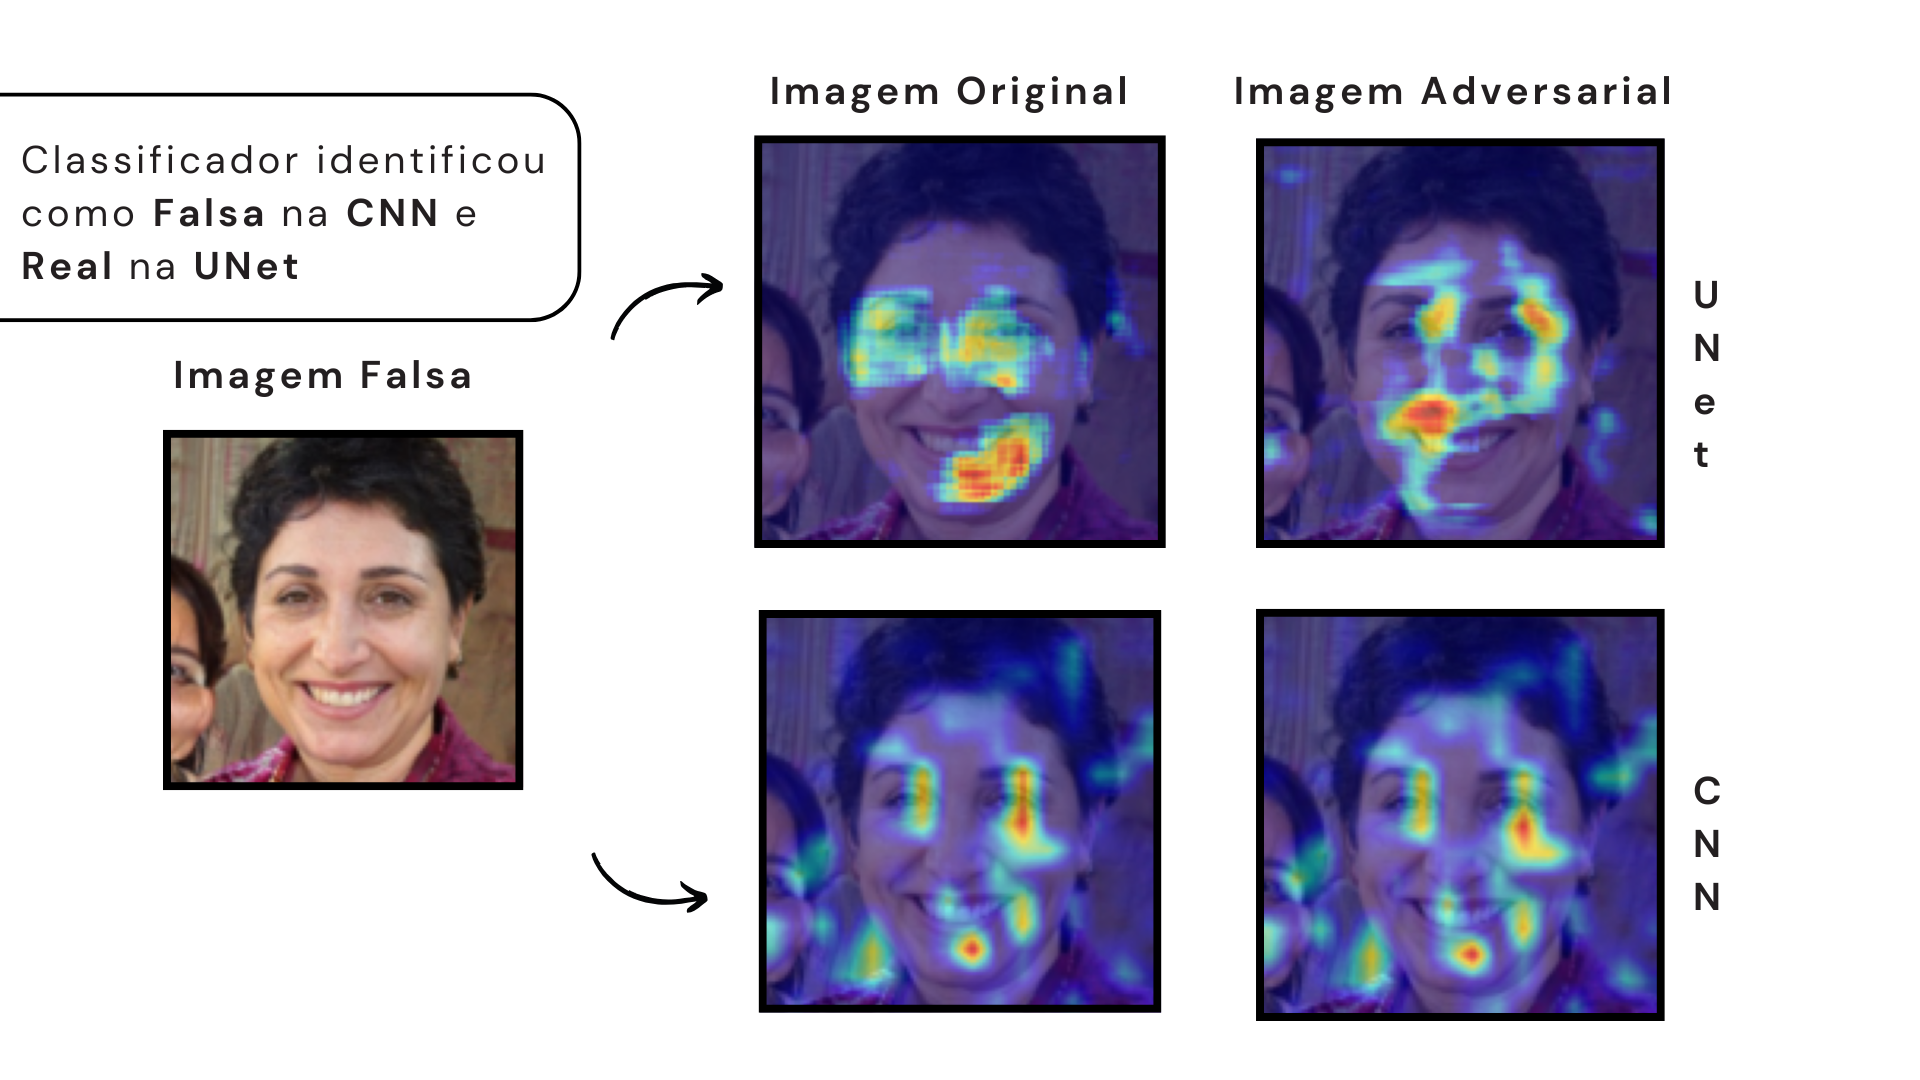
\includegraphics[width=1\textwidth]{figs/gradcam-imagem-falsa.png}
    \caption{Exemplos de visualização GradCAM para UNET e CNN com comparativo de imagem original e imagem adversarial.}\label{fig:gradcam_imagem_falsa}
\end{figure}

Nota-se que, para a rede neural da UNET, após a imagem ter sido alterada pela
rede adversarial, houve uma grande alteração nas áreas de interesse da rede.
Isso indica que a rede adversarial possui uma maior facilidade em alterar os
resultados esperados pelo classificador. Já no caso da CNN, as regiões de
interesse apenas foram realçadas, o que pode indicar uma maior robustez contra
ataques, obrigando a rede adversarial a gerar perturbações mais refinadas e
focalizadas, de modo a comprometer mesmo as regiões reforçadas pela CNN, o que
requer ajustes mais precisos nos parâmetros de otimização para induzir mudanças
significativas na decisão final do classificador.

\begin{figure}[htb]
    \centering
    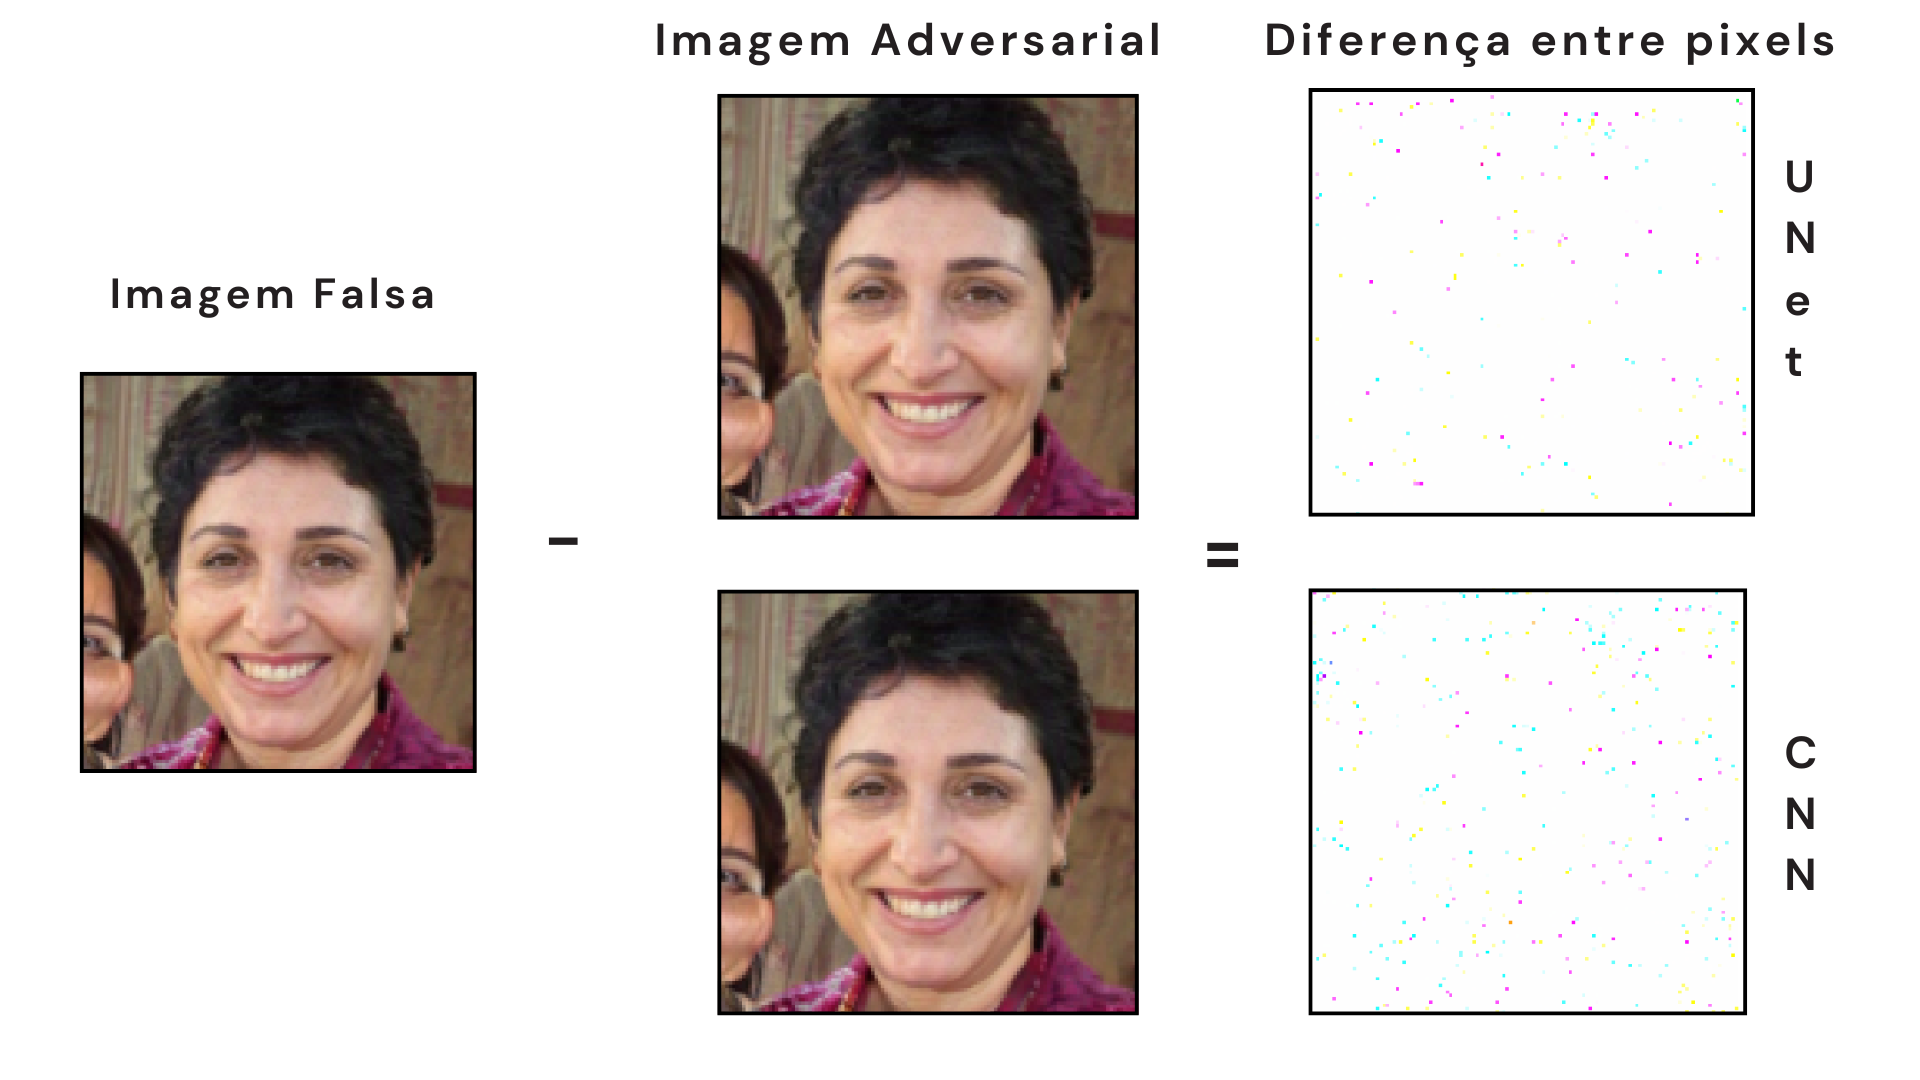
\includegraphics[width=1\textwidth]{figs/pixels-diff-imagem-falsa.png}
    \caption{Exemplos de imagens adversariais geradas pela CNN e UNET e a diferença no que foi alterado com base na imagem original }\label{fig:pixels_diff_imagem_falsa}
\end{figure}

Por fim, a Figura~\ref{fig:pixels_diff_imagem_falsa} ilustra as diferenças
entre a imagem adversarial e a imagem original. Nota-se que ambas as imagens
apresentam ruídos imperceptíveis a olho nu, atingindo o objetivo de gerar uma
imagem cuja alteração não seja detectada pelo observador. Ademais, observa-se
que cada gerador aprende um padrão distinto, o que pode explicar as
discrepâncias entre os resultados da avaliação cruzada
(Tabela~\ref{tab:resultados_cruzada}) e os obtidos na avaliação direta sob
ataque adversarial (Tabela~\ref{tab:resultados_metricas}).

\section{Conclusão}

Este trabalho teve como objetivo investigar a vulnerabilidade e a robustez de
diferentes classificadores de imagens faciais diante de ataques adversariais
imperceptíveis, além da análise da transferibilidade de vulnerabilidade entre
modelos Deep Learning distintos. A aplicação do ataque adversarial demonstrou
que perturbações sutis podem degradar significativamente o desempenho dos
classificadores, sobretudo das redes neurais, como indicado pelas expressivas
reduções de acurácia e pelos baixos índices de recall. Além disso, os mapas de
calor gerados via GradCAM evidenciaram que as áreas de interesse dos modelos,
tais como olhos e lábios, foram alteradas de maneira distinta, dependendo da
arquitetura. Em particular, a CNN mostrou uma robustez relativa maior, pois
suas regiões de atenção foram apenas realçadas, enquanto a versão reduzida da
UNET evidenciou uma maior facilidade para alterar os resultados esperados,
refletindo vulnerabilidades mais acentuadas.

Além disso, a avaliação cruzada dos ataques adversariais revelou que as
perturbações possuem propriedades transferíveis entre os modelos, embora a
eficácia do ataque varie conforme a arquitetura-alvo e não tenha atingido uma
redução tão considerável quanto os ataques não cruzados. Esses resultados
enfatizam não apenas as limitações dos métodos de classificação atuais, mas
também a necessidade de desenvolver estratégias defensivas mais robustas que
possam mitigar os impactos desses ataques em aplicações críticas, como o
reconhecimento facial.

Por fim, este estudo contribuiu para uma compreensão mais aprofundada das
vulnerabilidades presentes em sistemas baseados em aprendizado profundo,
evidenciando que mesmo perturbações imperceptíveis ao olhar humano podem
comprometer a integridade dos resultados. Destaca-se a importância de se adotar
mecanismos defensivos e de se explorar novas técnicas de treinamento que
considerem a adversarialidade como parte integrante do processo de aprendizado,
visando aumentar a resiliência dos modelos.

\bibliographystyle{sbc}
\bibliography{sbc-template}
\nocite{*}
\end{document}
